\documentclass[italian,12pt,a4paper]{article}
\usepackage[utf8]{inputenc}
\usepackage[T1]{fontenc}
\usepackage{babel}
\usepackage{graphicx}
\usepackage{subfig}
\usepackage{hyperref}
\usepackage{tikz}
\usepackage{pgf-pie}
\usepackage{algorithm}
\usepackage{algpseudocode}
\usepackage{algorithmicx}
\usepackage{placeins}
\usepackage{svg}
\usepackage{tabularx}
\definecolor{myblue}{rgb}{0.152,0.690,0.894} %39,176,228
\definecolor{mygrey}{rgb}{0.062, 0.419,0.639}
\title{Università degli studi di Bari facoltà di scienze MM.FF.NN}
\date{} % clear date
\hypersetup{
	colorlinks=true,
	linkcolor=black,
	filecolor=magenta,      
	urlcolor=cyan,
	pdfpagemode=FullScreen,
}
\graphicspath{ {./images/} }
\RequirePackage[subfigure]{tocloft}

\cftsetindents{section}{0em}{2em}
\cftsetindents{subsection}{0em}{2em}

\renewcommand\cfttoctitlefont{\hfill\Large\bfseries}
\renewcommand\cftaftertoctitle{\hfill\mbox{}}

\algrenewcommand\algorithmicrequire{\textbf{Input:}}
\algrenewcommand\algorithmicensure{\textbf{Output:}}

\setcounter{tocdepth}{2}
\begin{document}
	\maketitle
	\thispagestyle{empty}
	\begin{center}
		\huge	\textbf{Progetto Data Mining} \\
		\Large \textbf{NASA - Nearest Earth Objects hazard detection}
	\end{center}
	
	
	
	\begin{center}
		by \\
		\Large \textbf{Vito Proscia mat. 735975}
	\end{center}

	
	\begin{figure}[hb]
		\centering
		
\includegraphics[width=5cm]{image.png}
	\end{figure}
	
	\vfill
	\begin{center}
		Anno accadenico 2022-2023
	\end{center}
	
	\newpage
	
	\tableofcontents

	\newpage

	
	\section{Introduzione}

	\subsection{Contesto}

	\href{https://www.kaggle.com/datasets/sameepvani/nasa-nearest-earth-objects/}{Near-Earth Objects} (NEO) dataset contiene una serie di informazioni, raccolte dalla NASA, che caratterizzano degli oggetti rilevati vicino alla terra, molti di questi oggetti sono a migliaia di chilometri dalla superficie terrestre, ma su scala astronomica queste distanze sono molto piccole e possono influenzare fenomeni naturali, quali per esempio cambiamenti nella marea, eventi sismici, cambiamento atmosferico, variazioni magnetiche e così via. \\
	È importante sottolineare che la maggior parte degli corpi celesti che passano vicini alla Terra sono di piccole dimensioni e passano ad una distanza sicura, solitamente non hanno un impatto significativo sui fenomeni naturali, ma quelli di dimensioni maggiori o che si avvicinano molto possono avere degli effetti. \\
	\linebreak
	La natura dei Near-Earth Objects (NEO) si può dividere in:
	\begin{itemize}
		\item \textbf{Comete}: corpo celeste relativamente piccolo, composto da gas ghiacciati frammenti di rocce e metalli
		\item \textbf{Asteroidi}: corpi minori di un sistema planetario originati dallo stesso processo di formazione dei pianeti ma le cui fasi di accrescimento si sono interrotte più o meno presto, oppure formati attraverso la collisione tra altri corpi celesti, sono composti principalmente da silicati di nichel, ferro e magnesio
	\end{itemize}

	
	\subsection{Definizione obiettivo principale}
	L'obiettivo principale del progetto è quello di addestrare un modello per andare a predirre, in base ad alcuni parametri, quali corpi celesti rilevati attorno alla terra possono provocare danni, questo perchè è ormai ampiamente accettato dalla comunità scientifica che le collisioni di asteroidi con la Terra avvenute in passato hanno avuto un ruolo significativo nel disegnare la storia geologica e biologica del pianeta, per questo risulta interessante effettuare un task di classificazione binaria che coinvolge la feature \textit{hazardous} con classi:
	\begin{itemize}
		\item \textbf{True}: oggetto potenzialmente pericoloso
		\item \textbf{False}: oggetto non pericoloso
	\end{itemize}
	Inoltre si vogliono comparare le prestazioni di vari modelli addestrati con tecniche diverse per evidenziare la differenza nell'addrestamento utilizzando un dataset fortemente sbilanciato.
	In particolare si applicheranno tecniche di bilianciamento delle classi (resampling) che agiscono sui dati e tecniche di addestramento che vanno a considerare lo sbilanciamento (cost-sensitive learning) che riguardano più la controparte algoritmica. 
	
	
	\subsection{Tool utilizzati}
	Per la sperimentazione sono stati usati diversi stumenti, quali:
	
		\begin{itemize}
			\item \href{https://colab.research.google.com/}{Google Colab}, strumento  presente nella suite Google che consente di scrivere python notebook direttamente dal proprio browser, utilizzando risorse messe a disposizione da remoto. 
			\item \href{https://www.cs.waikato.ac.nz/~ml/weka/}{Weka}, software contenente una collezione di algoritmi per data Mining e apprendimento Automatico, scritto in Java e sviluppato presso University of Waikato New Zealand
			
		\end{itemize}


	\section{Analisi del dataset}
	
	\subsection{Descrizione features}
	Il dataset inizialmente si compone di 90836 osservazioni per dieci features che vanno a descrivere una serie di caratteristiche dei corpi celesti registrati, in particolare abbiamo:
	
	\begin{enumerate}
		\item \textit{id} [numeric]: identificatore univoco per ogno oggetto
		\item \textit{name} [string]: nominativo dato dalla NASA
		\item \textit{est\_diameter\_min} [numeric]: diametro minimo stimato (Km)
		\item \textit{est\_diameter\_max} [numeric]: diametro massimo stimato (Km)
		\item \textit{relative\_velocity} [numeric]: Velocità relativa rispetto alla terra (Km/h)
		\item \textit{miss\_distance }[numeric]: ???
		\item \textit{orbiting\_body} [string]: Corpo rispetto al quale l’oggetto sta orbitando
		\item \textit{sentry\_object} [boolean]: Copro incluso o meno in sentry (sistema di monitoraggio automatico delle collisioni)
		\item \textit{absolute\_magnitude} [numeric]: descrizione della luminosità dell’oggetto (energia radiata dal corpo al secondo)
		\item \textit{hazardous} [boolean]: Indica se il corpo è pericoloso o meno
	\end{enumerate}
	
	\subsection{Preparazione dati}
	
	\subsubsection{Analisi delle input features}
	Andando a considerare direttamente il dataset come ci vine fornito ci sono una serie di problematiche legate ad alcune features, alcune di queste sono inutili per lo scopo di addestramento, quali: 
	
	\begin{itemize}
		\item \textit{id} (nessuna correlazione con la feature su cui fare predizione),
		\item \textit{name} (nessuna correlazione con la feature su cui fare predizione), 
		\item \textit{orbiting\_body} (ha un unico valore)
		\item \textit{sentry\_object} (ha un unico valore)
	\end{itemize}
	
	Un'altra considerazione si potrebbe fare sulle features \textit{est\_diameter\_min} e \textit{est\_diameter\_max}, andando a descrivere la dimensione di diametro massima e minima, si potrebbero accopare i dati delle due caratteristiche con un'unica che andrebbe a rappresentare la media matematica dei due valori (\textit{est\_diameter\_mean}).
	
	
	\subsubsection{Analisi della target feature}
	
	Il "problema" più grande del lavoro riguarda la natura delle osservazioni inerenti alla target feature \textit{hazardous}, che presenta una distrubuzione di valori fortemente sbilanciata ($90.3\%$ per false e $9.7\%$ per True)
	\\
	\linebreak
	\linebreak
	\begin{center}
	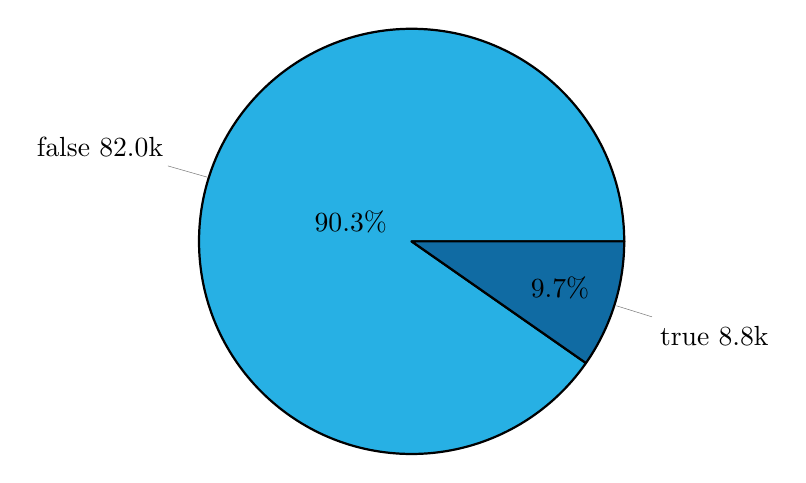
\begin{tikzpicture}[scale=0.9]
		\pie[color={myblue, mygrey}, text=pin]{90.3/false 82.0k, 9.7/true 8.8k}
	\end{tikzpicture}
\end{center}

	\section{Resampling per lo sbilanciamento delle classi}
	Il resampling è un tecnica (data focsed) usata per bilanciare le osservazioni di ogni classe andando a generarne di nuove o eliminandole per risolvere il problema dello sblianciamento.
	
	\subsection{Oversampling vs Undersampling}

	L’oversampling e l’undersampling sono due metodi per andare a risolvere lo sbilanciamento delle classi target, in particolare l’undersampling prevede il ridimensionamento di una classe prelevando da una popolazione un suo sottoinsieme, questo si applicherebbe alla classe più numerosa, mentre l’oversampling sposta il focus sulla classe con meno occorrenze andando a creare “sinteticamente” delle nuove osservazioni a partire da quelle già a disposizione.
	
	\subsection{Approccio ibrido}
	Nel nostro caso, come già accennato, le classi della target feature \textit{hazardous} (true/false) sono molto sbilanciate (causa del fatto che per fortuna sono pochi i corpi celesti che si rivelano potenzialmente pericolosi), se da una parte i \textit{false} superano gli 80k, dall'altra i \textit{true} arrivano a malapena a 8k, quindi se applicassimo una tecnica di undersampling si avrebbe un’enorme perdita di informazioni, mentre se usassimo l’oversampling, per bilanciare i dati avremo moltissimi dati sintetici, per questo sarebbe meglio usare una tecnica ibrida.
	\linebreak
	\subsubsection{SMOTE-ENN}
	L’algoritmo SMOTE-ENN [Batista et al 2004] combina l’abilità di SMOTE (Synthetic Minority Oversampling)  di generare istanze sintetiche per la classe minoritaria, con quella di ENN (Edited Nearest Neighbor) [Wilson 1972] di eliminare da entrambe le classi alcune osservazioni. \\
	\linebreak
	L'algoritmo, come dice il nome, è basato su SMOTE, tecnica usata per la creazione di istanze sintetiche della classe minoritaria, andando a aggiungere nuove istanze con valori mediati tra i $k$ vicini di una osservazione della classe, prorpio per questo, teoricamente, nella nostra situazione non dovrebbe performare troppo bene, avendo le istanze della classe minoritaria molto vicine a quella della classe maggioritaria, creando così istanze sintetiche con valori mediati tra classi diverse.
	
	\begin{algorithm}
		\caption{SMOTE-ENN}
		\begin{algorithmic}
			\Require $Tr$ : Training set, \\ $p$: number of nearest neighbors in SMOTE, \\ $k$: number of nearest neighbors in ENN
			\Ensure $New\_Tr$ : Training set after using SMOTE-ENN \\
			\textbf{1.} Divide $Tr$ into positive and neative subsets: \\ $Tr \leftarrow Pos \cup Neg;$  \\
			\textbf{2}. Oversampling the minority class using SMOTE to balance calss distribution: \\
			$New\_Pos \leftarrow SMOTE(Pos, p);$ \\
			$|New\_Pos| = |Neg|;$ \\
			\textbf{3.} $New\_Tr \leftarrow New\_Pos \cup Neg;$ \\
			\textbf{4.} Remove noisy examples using ENN: \\
			$New\_Tr \leftarrow ENN(New\_Tr);$
		\end{algorithmic}
	\end{algorithm}

	\begin{figure}[!ht]
		\centering
		\subfloat[Prima di SMOTE-ENN]{%
			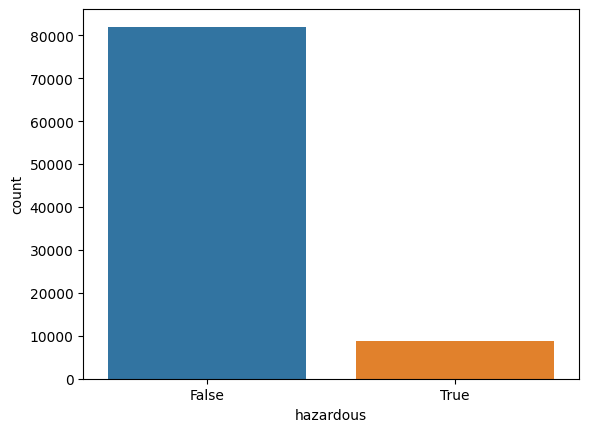
\includegraphics[scale=0.5]{output1.png}%
		}%
		\subfloat[Dopo SMOTE-ENN]{%
			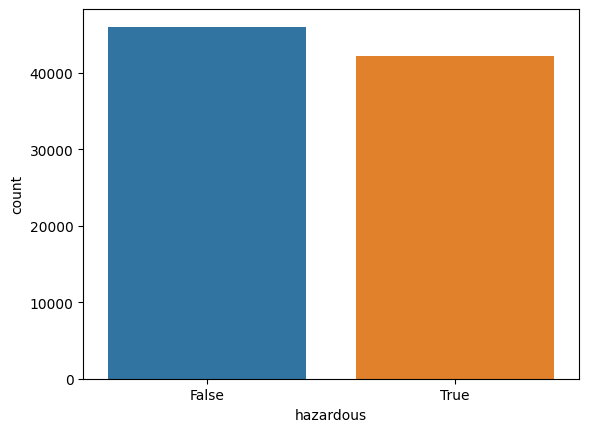
\includegraphics[scale=0.5]{output2.png}%
		}%
	\end{figure}
	\subsubsection{ADASYN}
	L'algoritmo ADASYN (Adaptive Synthetic) si basa sull'idea di generare sinteticamente dei nuovi dati per la classe minoritaria considerando la distribuzione delle osservazioni della sudetta classe. Vengono geneari più dati a partire dalle osservazioni, della classe minoritaria, che sono più dififcili da imparare. \\
	La chiave di ADASYN è l'uso della distribuzione dei pesi $\hat{r_i}$ come criterio per decidere quante osservazioni sintetiche creare per ogni esempio della classe minoritaria.
	
		\begin{algorithm}
		\caption{ADASYN}
		\begin{algorithmic}
			\Require $Tr$ : Training set, \\ $m\_s$: number of samples of minority class, \\ $m\_l$: number of samples of majority class.
			\Ensure $Tr\_res$ : Training set resampled \\
			\textbf{1.} Calculate the degree of class imbalance: $$d = \frac{m_s}{m_l} \in (0, 1]$$  \\
			\textbf{2}. \textbf{If} {$d < d_{th}$} ($d_{th}$ preset threshold) \\
						\quad\textbf{a)} Calculate the number of synthetic data examples that
						need to be generated for the minority class: $$G = (m_l - m_s)\beta$$
						\quad Where $\beta \in [0, 1]$ balance level after generation of the synthetic data. \\
						\quad \textbf{b)} \textbf{For each} example $x_i \in minorityClass$ find $k$ nearest neighbors and calculate: $$r_i = \frac{\Delta_i}{k} = \frac{\# majotiry\_class\_neighbors}{k}, i = 1, \dots m_s$$
						\quad \textbf{c)} Normalize $r_i$ according to: $$\hat{r_i} = \frac{r_i}{\sum_{j = 1}^{m_s} r_j}$$
						\quad \textbf{d)} Calculate the number of synthetic data examples for each $x_i$: $$g_i = \hat{r_i} G$$
						\quad \textbf{e)} \textbf{For} $1$ \textbf{to} $g_i$ \\
						\quad \quad \textbf{i)} Randomly choose one minority data example, $x_{zi}$,
						from the $k$ nearest neighbors for data $x_i$ \\
						\quad \quad \textbf{ii)} Generate the synthetic data example: $$s_i = x_i + (x_{zi} - x_i)\lambda$$
						Where $(x_{zi} - x_i)$ is the difference vector and $\lambda \in [0,1]$ is a random number. \\

		\end{algorithmic}
	\end{algorithm}
	\begin{figure}[!ht]
	\centering
	\subfloat[Prima di ADASYN]{%
		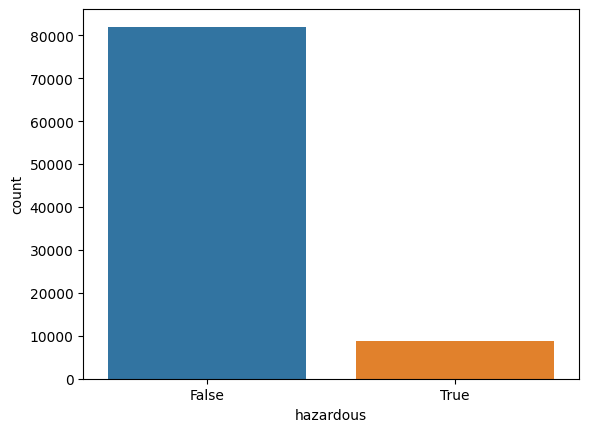
\includegraphics[scale=0.5]{output1.png}%
	}%
	\subfloat[Dopo ADASYN]{%
		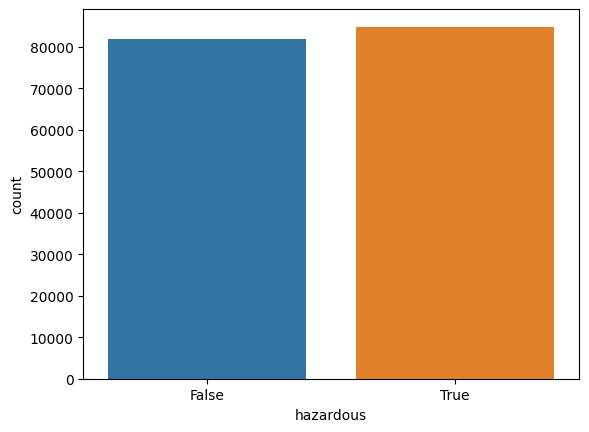
\includegraphics[scale=0.5]{output3.png}%
	}%
\end{figure}
	
	\section{Cost-Sensitive learning per lo sbilanciamento delle classi}
	Il \textit{cost-sensitive learning} è un task di data mining che tiene in considerazione il costo di una classificazione sbagliata (\textit{misclassification cost}), andnado a considerare una classificazione binaria, ad ogni tipo di predizione viene asseganto un costo, formando una \textit{cost matrix}: \\
	\begin{center}
		\begin{tabularx}{0.8\textwidth} { 
				| >{\centering\arraybackslash}X 
				| >{\centering\arraybackslash}X 
				| >{\centering\arraybackslash}X | }
			\hline
			 & Actual negative & Actual positive \\
			\hline
			Predict negative & $C(0, 0)$ TN & $C(0, 1)$ FN \\
			\hline
			Predict positive  & $C(1, 0)$ FP & $C(1, 1)$ TN \\
			\hline
		\end{tabularx}
	\end{center}

	Dove $C(i, j)$ rappresenta il costo della classificazione dove $i$ è la predizione, mentre $j$ è la classe corretta. \\
	Il cost-sensitive learning è utile in caso di sbilanciamento delle classi perchè da più peso agli errori di classificazione, in particolare nella classificazione dei FN (False Negative) cioè esempi classificati come \textit{false} ma che in realtà sono \textit{true}.
	
	\subsection{Threshold factor}
	Il \textit{threshold factor} è un valore che consente la classificazione di una osservazione $x$ in \textit{true} (assumendo che la classe minoritaria sia quella con valori \textit{true}).
	\linebreak
	In particolare: $$p* = \frac{FP}{FP + FN} = \frac{C(1, 0)}{C(1, 0) + C(0, 1)}$$
	Se $P(true, x) \ge p*$ allora $x$ viene classificato come \textit{true}.
	
	\subsubsection{Meta Learning}
	Il \textit{meta learning} è un tipo di \textit{cost-sensitive learning} che converte un algoritmo \textit{cost-insensitive} in uno \textit{cost-sensitive} in due modi diversi:
	
	\begin{itemize}
%		\item \textbf{Threshold}, usa la soglia $p*$ per la classificazione
		\item \textbf{Sampling}, modifica della distribuzione dei dati per poi andare ad applicare un algoritmo di learning
	\end{itemize}
	
	\section{Machine Learning}
	Tenendo conto di tutte le considerazioni fatte, la parte inerente all'addestramento ed alla successiva valutazione si concentrerà in particolare sulle differenze tra l'addestramento su tre instanze del dataset, in particolare con il dataset originale, il dataset su cui è eseguito l'algorimto SMOTE-ENN ed il dataset su cui è eseguito ADASYN, andando a differenziare tra cost-insensitive learning e cost-sensitive learning.
	
	
		\begin{figure}[hb]
			\centering
			\includegraphics[width=15cm]{untitled2}
		\end{figure}
		
	\subsection{Modelli di learning}
	L'addestramento avverrà principalmente con due modelli di learning:
	
	\begin{itemize}
		\item Albero di decisione, in particolare il C4.5
		\item Naive Bayes, in particolare la variante Complement Naive Bayes (particolarmente utile per dati sbilanciati)
	\end{itemize}
	   
	\subsubsection{Decision Tree C4.5}
	Modello di classificazione che prende in input una collezione di esempi di training $S$ e l'iniseme delle classi $C = \{c_1, c_2, \dots, c_k\}$, ad ogni nodo dell'albero, C4.5 sceglie l'attributo dei dati che più efficacemente suddivide $S$ insieme di campioni in sottoinsiemi in base alle classi. Il criterio di suddivisione è \textit{l'information gain} (differenza di entropia). L'attributo con il più alto guadagno di informazioni normalizzate viene scelto per prendere la decisione. \\
	\textit{l'information gain} per l'attributo di test $t$ sarà:
	
	$$IG(S, t) = E(S) - \sum_i \frac{|S_i|}{|S|}E(S_i)$$ dove $$E(S) = -\sum_{i = 1, \dots, k} Count(c_i, S)\cdot\log(Count(c_i, S))$$
	
	Nel nostro caso abbiamo applicato allenato il modello con sei configurazioni:
	
	\begin{itemize}
		\item \texttt{DecisionTreeClassifier().fit(X\_train, y\_train)}, classificatore cost-insensitive addesstrato su il dataset originale, il dataset ribilanciato con SMOTEENN e il dataset ribilanciato con ADASYN.
		\item \texttt{DecisionTreeClassifier(class\_weight="balanced").fit(X\_train, y\_train)}, classificatore cost-sensitive addesstrato su il dataset originale, il dataset ribilanciato con SMOTEENN e il dataset ribilanciato con ADASYN.
		
	\end{itemize}
	
	N.B. L'attributo \texttt{class\_weight} è stato impostato a \texttt{"balanced"} per andare a regolare automaticamente i pesi in modo inversamente proporzionale alle classi: $$w_{true} = \frac{N_s}{2\cdot N_{true}} \quad w_{false} = \frac{N_s}{2\cdot N_{false}}$$ dove $N_s$ è la cardinalità del dataset, $2$ rappresenta il numero di classi, $N_{true}$ e $N_{false}$ sono rispettivamente il numero di occorrenze con classe \textit{true} e della classe \textit{false}.
	
	
	
	%\subsection{Riduzione del rumore nei dati}
	%I dati rumorosi sono privi di significato, che vanno ad inficiare le performance dei modelli allenati su di essi, per questo è sempre meglio ridurili, la presenza di rumore nei dati può essere dovuta a molteplici fattori, per es. il mancato funzionamento dei sensori che raccolgono dati, errori di programmazione, input incomprensibi e così via.
%	Nel nostro caso il rumore si esprime attravero istanze duplicate e presenza di outlier. \\
	%\linebreak
	%Per andare a rimuovere i duplicati possiamo fare ricorso ad un fltro di \texttt{weka}, in particolare: \texttt{weka.filters.unsupervised.instance.RemoveDuplicates}, passando da 88283 osservazioni a 88253. \\
	%\linebreak
%	Per quanto riguarda gli outliers
	
	\subsubsection{Naive Bayes}
	




	\section{Analisi esplorativa dei dati}

	\section{Conclusioni}
	

	
\end{document}